\documentclass[11pt]{article} % For LaTeX2e
\usepackage{manuscript, palatino}
\usepackage{graphicx}
\usepackage{hyperref}
\usepackage{amsfonts, amsmath}
\usepackage{algorithm, algpseudocode}%
\usepackage[numbers,super]{natbib}

\title{Anxiety, avoidance, and sequential evaluation}

\author{
Samuel Zorowitz \\
Princeton Neuroscience Institute\\
Princeton University\\
Princeton, NJ 08540 \\
\texttt{zorowitz@princeton.edu} \\
\And
Ida Momennejad \\
Columbia University\\
New York, NY 10027 \\
\texttt{ida.m@columbia.edu} \\
\And
Nathaniel D. Daw \\
Princeton Neuroscience Institute\\
and Department of Psychology\\
Princeton University\\
Princeton, NJ 08540 \\
\texttt{ndaw@princeton.edu} \\
}

\newcommand{\fix}{\marginpar{FIX}}
\newcommand{\new}{\marginpar{NEW}}

\begin{document}

\maketitle

\begin{abstract}
Anxiety disorders are characterized by a range of aberrations in the processing and response to threat, but there is little clarity what core pathogenesis might underlie these symptoms. Here we propose a decision theoretic analysis of maladaptive avoidance and embody it in a reinforcement learning model, which shows how a localized bias in beliefs can formally explain a range of phenomena related to anxiety. The core observation, implicit in standard decision theoretic accounts of sequential evaluation, is that avoidance should be protective: if danger can be avoided later, it poses no threat now. We show how a violation of this assumption --- a pessimistic, false belief that later avoidance will be unsuccessful --- leads to a characteristic propagation of fear and avoidance to situations far antecedent of threat. This single deviation can explain a surprising range of features of anxious behavior, including exaggerated threat appraisals, fear generalization, and persistent avoidance. Simulations of the model reproduce laboratory demonstrations of abnormal decision making in anxiety, including in situations of approach-avoid conflict and planning to avoid losses. The model also ties together a number of other seemingly disjoint issues in anxious disorders. For instance, learning under the pessimistic bias captures a hypothesis about the role of anxiety in the later development of depression. The bias itself offers a new formalization of classic insights from the psychiatric literature about the central role of maladaptive beliefs about control and self-efficacy in anxiety. This perspective is importantly different from previous computational accounts of beliefs about control in mood disorders, which neglected the sequential aspects of choice.
\end{abstract}

\keywords{
anxiety; avoidance; fear generalization; decision theory; computational psychiatry
}

\acknowledgements{This research was supported in part by NIH grant MH10917, part of the CRCNS program.}

\startmain

\section{Introduction}

Though anxiety disorders differ in their particular symptomology, and in the content and situations which elicit anxious responding, they all are similarly characterized by aberrations in the processing of and response to threat\citep{dsm5}. In particular, at least three symptoms are manifest across the anxiety disorders. First, anxiety is associated with exaggerated threat appraisal, or a bias towards evaluating threat as disproportionately greater in likelihood and severity than is warranted\citep{ClarkBeck2011}. Second, anxiety is also associated with fear generalization, wherein the primary threat becomes associated with increasingly distal locations, events, and thoughts\citep{dymond2015}. Finally, anxiety is associated with persistent avoidance behavior, which often occurs well in advance of the materialization of actual threat\citep{Arnaudova2017}. Avoidance behaviors in anxiety are especially pernicious as they indirectly maintain anxiety by preventing learning from the non-occurrence of perceived threats. Though laboratory studies of decision making and learning in anxious populations have corroborated these clinical observations \citep{Harle2017, norbury2018, Aylward2019}, none offer an explanation as to the root of these symptoms.

These symptoms are particularly puzzling from a decision theoretic perspective\citep{huys2015}. Fear and avoidance of situations far in the future violates the basic logic of evaluation over sequential trajectories of action. Put another way, distant threat need not necessarily impinge on decision making in the present. This is because avoidance is by nature protective: the ability to successfully avoid danger in the future means an agent need not also do so now. For instance, cars endanger pedestrians but can be reliably avoided by following traffic signals; given that, staying indoors offers little or no additional protection from accidents. This is an instance of a general property of evaluation in sequential decision making: the value of present action turns fundamentally on assumptions about subsequent events, which include the agent's own subsequent choices. Typically, it is appropriate to assume that an agent will continue make good (i.e. reward-maximizing/harm-minimizing) choices down the line.

This line of reasoning hints that a fundamental deficit in anxiety disorders may relate to this assumption, which otherwise should preclude the spread of threat and excessive avoidance. Indeed, anxiety disorders are associated with pessimistic beliefs about the future \citep{ClarkBeck2011}. Clinically and subclinically anxious individuals judge future threat as more likely than do non-anxious individuals\citep{ButlerMathews1983, ButlerMathews1987, MacleodByrne1996}. Importantly, the development and maintenance of clinical anxiety is strongly tied to diminished perceived control\citep{bandura1977, barlow2002, gallagher2014a}, such that anxious individuals are more likely to endorse the belief that they are unlikely or unable to mitigate future threat. Indeed, a belief (or lack thereof) of one's ability to successfully navigate future danger is associated with anxiety\citep{davey1996, dugas1997}, and an increased belief in perceived control over threat is correlated with symptom reduction across the family of anxiety disorders\citep{gallagher2014b}. 

Here, we develop this idea into a model of evaluation under pessimistic assumptions about future choices. We show that a single, localized deviation can explain a surprising range of features of anxious behavior including exaggerated threat appraisal, fear generalization, and persistent avoidance. This account also offers a new formalization of classic insights from the psychiatric literature about the central role of beliefs about control and self-efficacy in anxiety \citep{bandura1977, barlow2002}. Specifically, we demonstrate a model with a misbelief in the reliability of future self-action gives rise to the anxious symptoms. Our perspective is importantly different from previous computational accounts of beliefs about control in mood disorders (e.g. \cite{HuysDayan2009}), which neglected the sequential aspects of choice.

\section{Model description}

We model anxious decision making in the context of Markov decision processes (MDPs). A standard normative assumption is that agents attempt to optimize the expected cumulative discounted reward,

\begin{equation*}
Q^\pi(s,a) = r(s,a) + \gamma \sum_{s'} p(s' \mid s,a) \sum_{a'} \pi(a' \mid s') Q^\pi(s',a'),
\end{equation*}

but for any particular state-action $a$, this is necessarily defined only relative to a policy $\pi(a' \mid s')$ specifying the assumed distribution of \emph{future} choices. The return can be optimized self-consistently under the assumption that the agent makes the return-maximizing choice at each step in the future, leading to the familiar expression for the optimal values,

\begin{equation}\label{eq:bellman}
 Q^*(s,a) = r(s,a) + \gamma \sum_{s'} p(s' \mid s,a) \max_{a'} Q^*(s',a').
\end{equation}

The ``max'' operator in Eq.~\ref{eq:bellman} yields a fundamental asymmetry between approach and avoidance, as illustrated in Fig.~1. The assumption that the agent makes the return-maximizing choice at each step implies that opportunities for reward propagate recursively to earlier steps, but avoidable dangers do not. This principle is highlighted in a toy MDP: a deterministic open gridworld with terminal states containing a single reward and punishment (Fig.~1a). The optimal state values $V^* = \max_a Q^*(s,a)$ (Fig.~1b) reflect a ``mountain'' of opportunity propagating recursively from the reward. Conversely, because harm is avoidable in this environment, its negative value is contained: all states (even those adjacent to threat) represent the opportunity for reward.

An agent is not restricted to the return-maximizing assumption, and could anticipate encountering danger under different assumptions about the future. For example, an agent may expect to fail to take the correct protective actions (i.e., expects to use a nonoptimal $\pi(a \mid s)$), or may expect the world's future dynamics do not guarantee reliable avoidance even so (i.e., under stochastic or adversarial transition dynamics $P(s' \mid s,a)$). Consider an agent who has such pessimistic expectations about dangerous events at future steps. Computing returns with such pessimistic predictions might help to quantify uncertainty in outcomes (i.e. to learn different points in the distribution of possible returns)\cite{bellemare2017}, and choosing on this basis can be adaptive in that it increases the chances of safety in uncertain or even adversarial scenarios\cite{Garcia2015}. 

Here we propose unrealistically pessimistic assumptions as a root cause of many anxious symptoms. Although such pessimism can be encoded either in the policy, $P(s' \mid s,a)$, or transition probabilities, $\pi(a \mid s)$, here for concreteness we work with distortions in the policy. In particular, we adopt the $\beta$-pessimistic value function from \cite{Gaskett2003}, to define an expectation of state-action value,

\begin{equation*}
Q^w(s,a) = r(s,a) + \gamma \sum_{s'} p(s' \mid s,a) \left( w \max_{a'} Q^w(s',a') + (1 - w) \min_{a'} Q^w(s',a') \right)
\end{equation*}

The parameter $w$ controls the degree of pessimism. An optimistic agent ($w = 1$) expects in the future to act fully in accordance with its preferences whereas a pessimistic agent ($w = 0$) expects to act contrary to its preferences. (We return to pessimism about state transitions in the discussion.) åFig.~1c,d illustrates the the consequences of different levels of pessimism for valuation in the example gridworld. An increasing expectation that the agent may fail to avoid in future causes the value of threat to permeate with increasing distance across the state space.

\begin{figure}
  \centerline{%
    \resizebox{1.0\textwidth}{!}{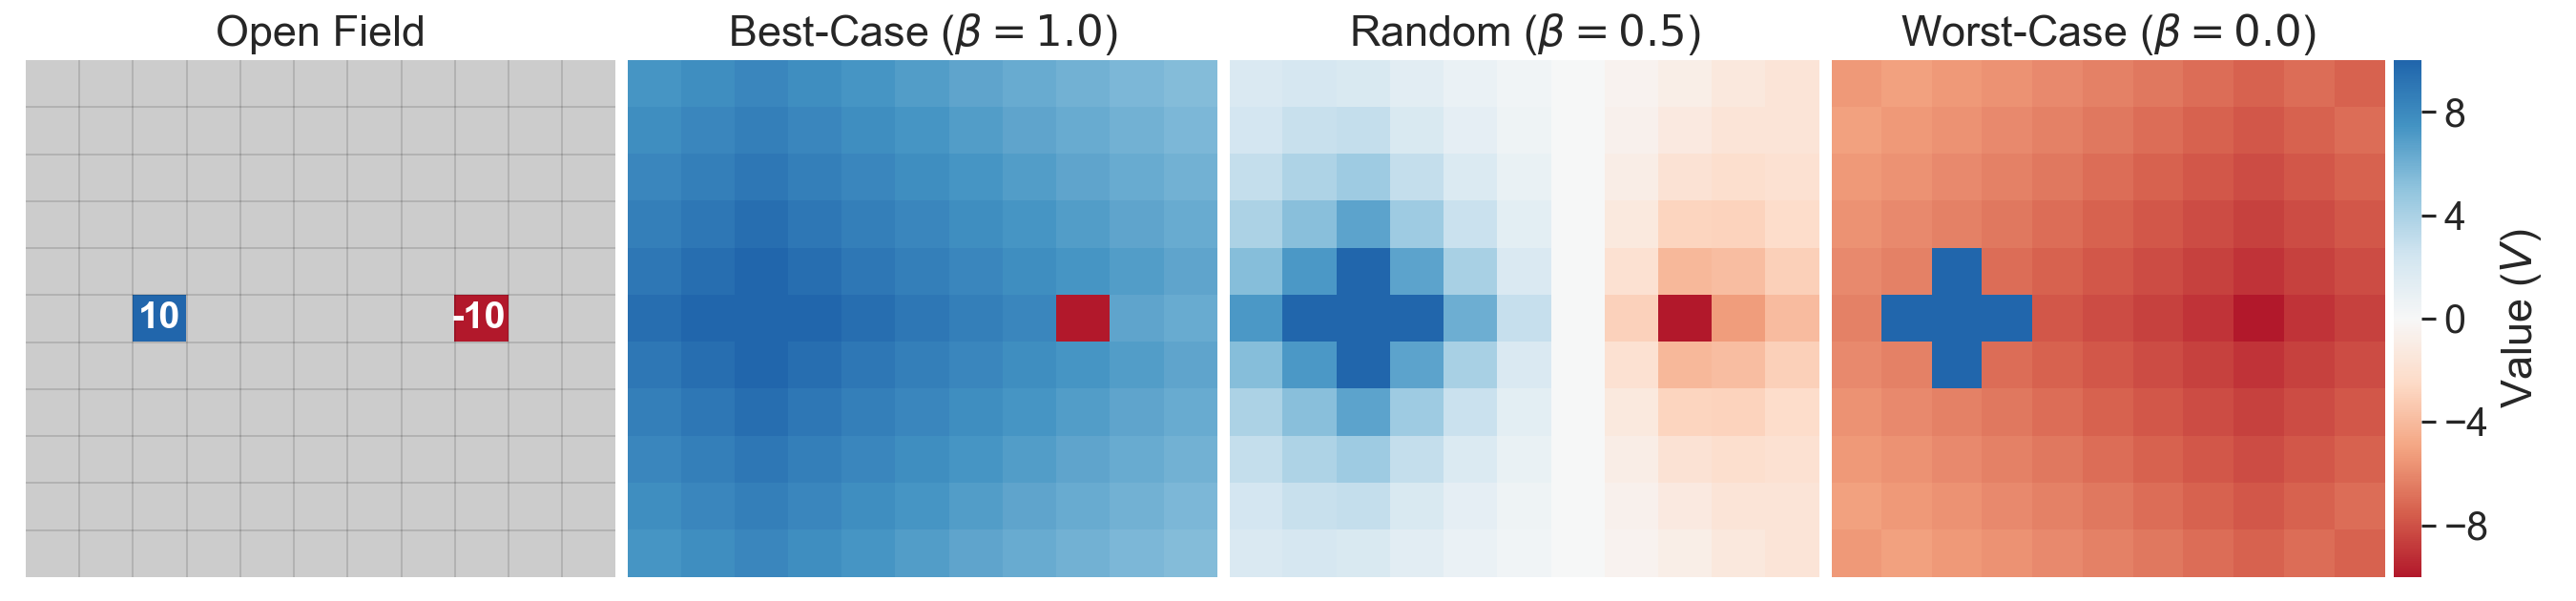
\includegraphics[trim={0 0 0 0},clip]{../../figures/01_field.png}}%
  }
  \par \textbf{Figure 1:} (A) A simple deterministic gridworld with two terminal states: one rewarding (blue) and one aversive (red). (B-D) States colored by their value under different levels of pessimism, with arrows showing an optimal trajectory. (B) For an optimistic agent ($w=1$), all states (other than the harmful state) take on positive value. (C) For a pessimistic agent ($w=0.5$), negative value spreads from the source to antecedent states. (D) With increasing pessimism ($w=0$), the extent of the spread grows worse. (Parameters: $\gamma = 0.95$)
\end{figure}

This simple simulation --- reflecting a localized violation of the core decision theoretic assumption of future return-optimizing action --- already echoes several core symptoms of anxiety disorders. Namely, the pessimistic agents in Fig~1c,d exhibit exaggerated threat appraisals (otherwise neutral states unrealistically signal danger); generalization of fear (threat value spreads across the gridworld); and persistent avoidance (early on, the agent takes paths which maintain increasing distances from threat). Importantly, as will be elaborated on below, this deviation from the usual assumptions is supported by prominent clinical theories of anxiety.

\section{Simulations}

In the following, we will demonstrate through simulation how our simple model can account for anxious behavior in laboratory-based studies of sequential learning and decision making. We will also show that our model is consistent with clinical theory describing the transition from clinical anxiety to depression. Unless otherwise noted, state and action values under varying degrees of pessimism were solved for using the value iteration dynamic programming method\citep{SuttonBarto2018}. All simulations were implemented in the Python programming language and the code is publicly available at \url{https://github.com/ndawlab/seqanx}. 

\subsection{Approach-avoidance conflict}

One behavioral finding characteristic of anxiety disorders is unbalanced processing of approach-avoidance conflict \citep{aupperle2010}; anxious individuals are more likely to forgo potential gains in order to avoid potential danger. Many of the disruptions anxiety causes to everyday functioning (e.g. avoiding social obligations for fear of possible social humiliation) can be understood in these terms. As such, many have sought to probe and measure this behavior in the laboratory. For instance, in the balloon analog risk task (BART) \citep{Lejuez2002}, participants attempt to earn money by pumping virtual balloons. With each pump, the balloon inflates and money is earned, but so too does the chance that the balloon pops and the accumulated earnings are lost. At any point in a trial, a participant may cash out, banking the money earned and ending the trial. Anxiety is correlated with fewer pumps of the balloon and earlier cash-outs in the BART \citep{Maner2007, ramirez2015}.

\begin{figure}
  \centerline{%
    \resizebox{1.0\textwidth}{!}{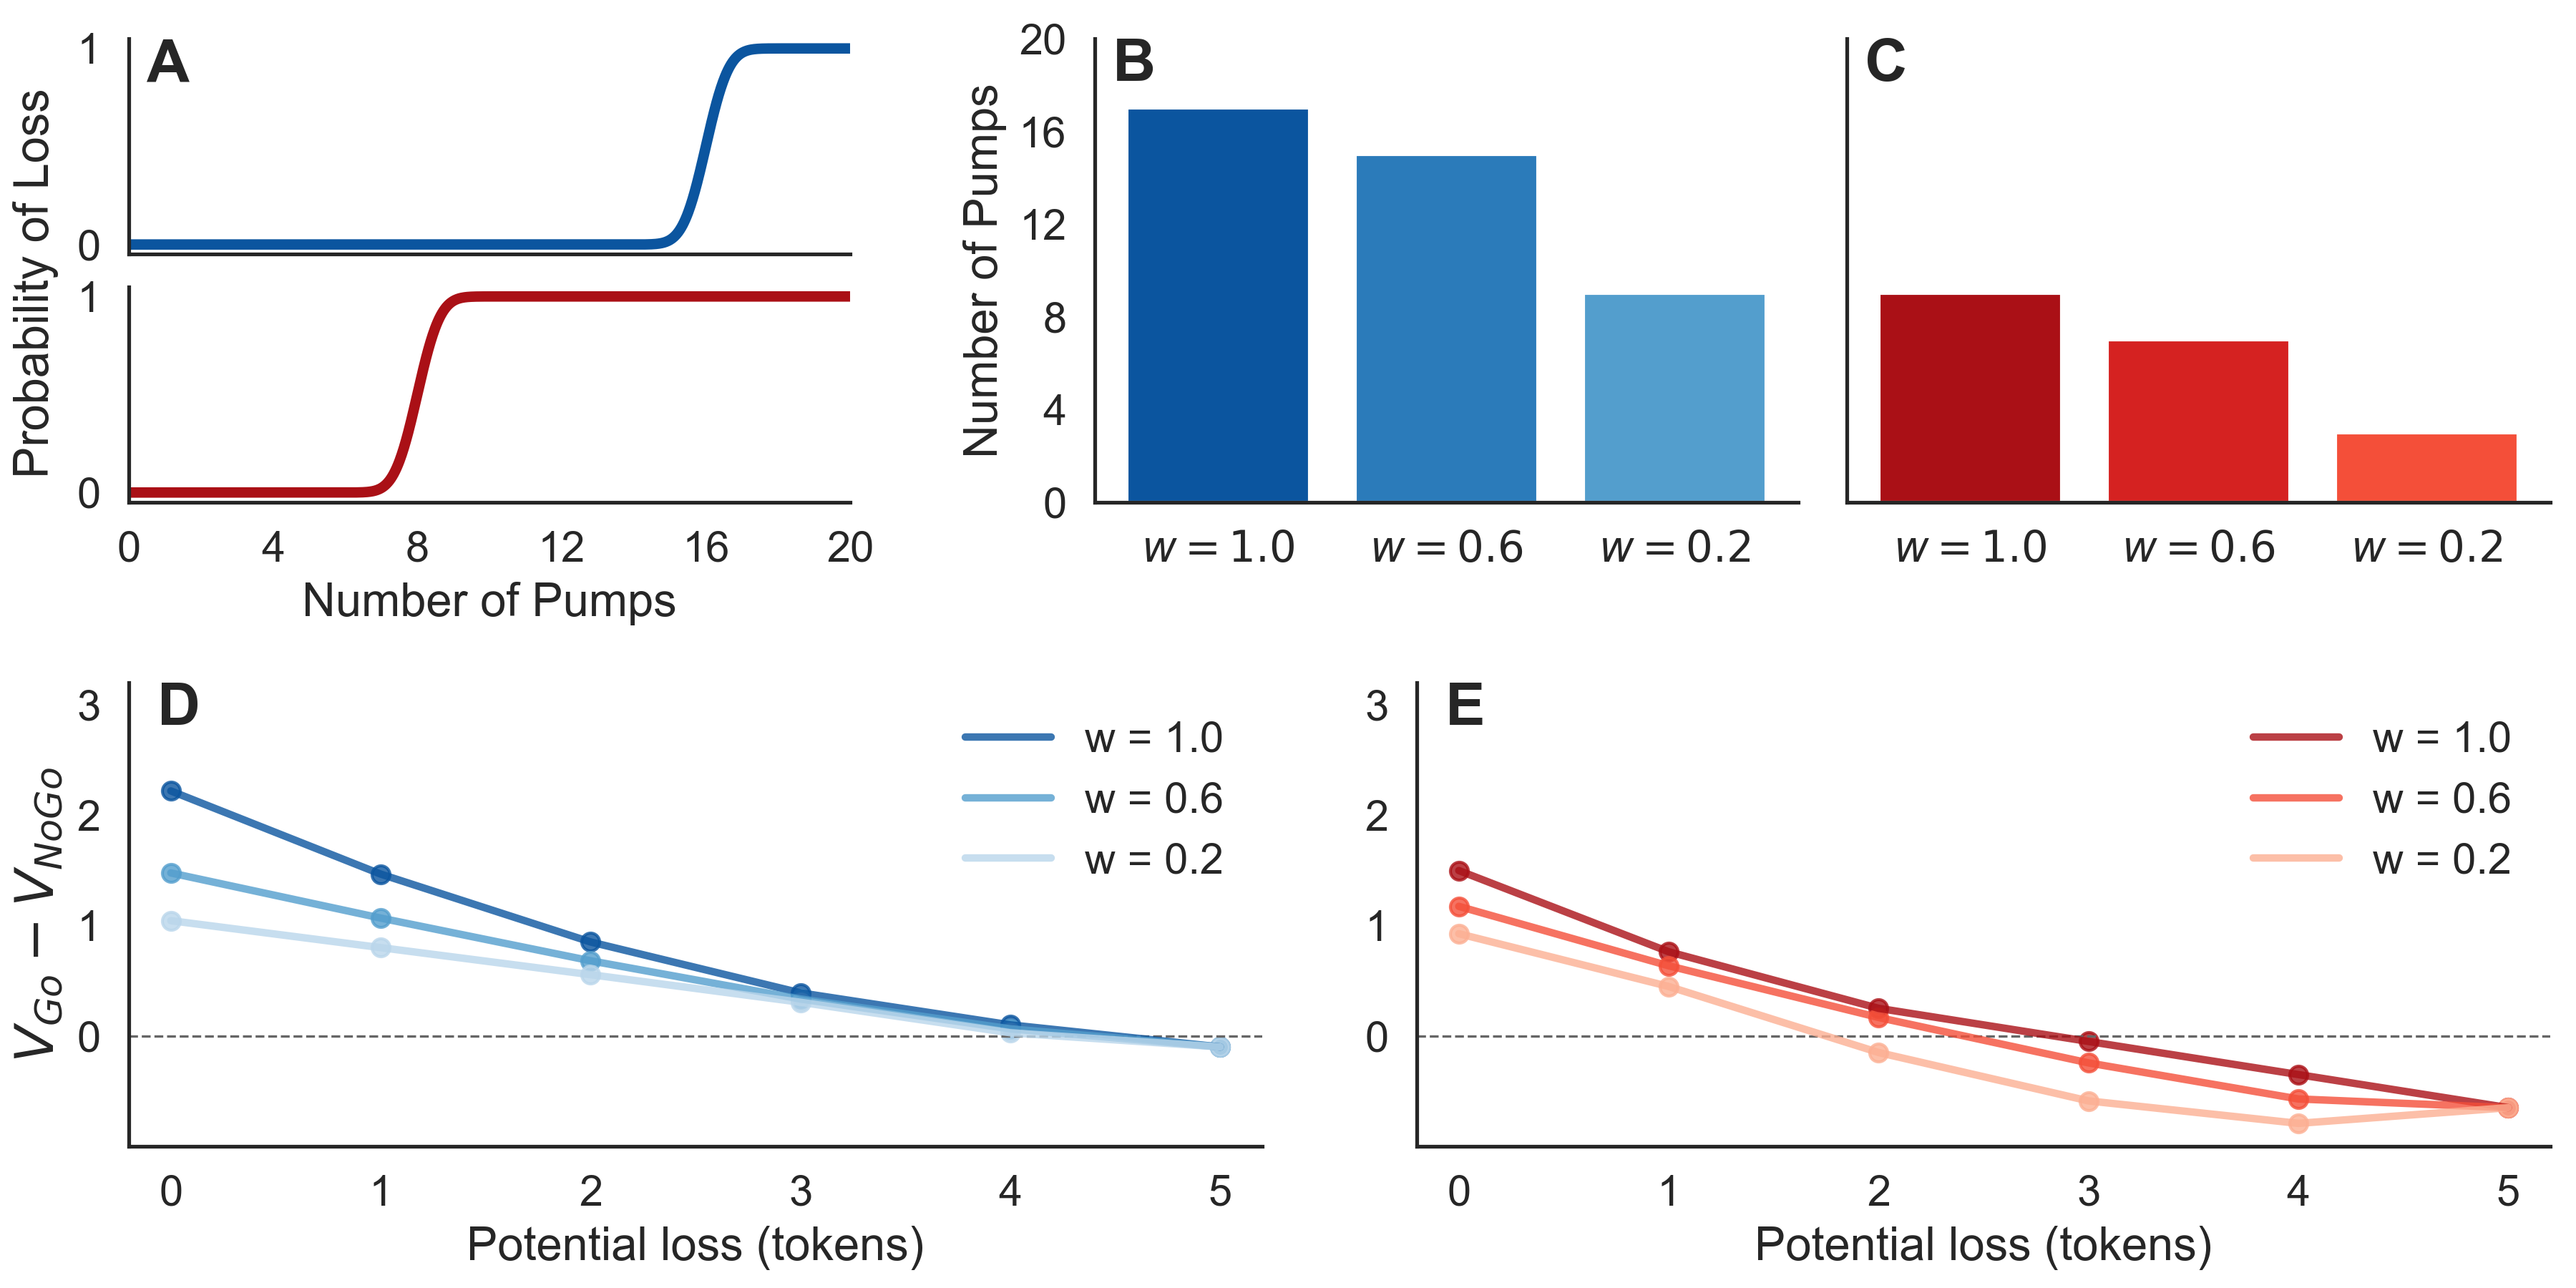
\includegraphics[trim={0 0 0 0},clip]{../../figures/02_appavo.png}}%
  }
  \par \textbf{Figure 2:} (A) The Balloon Analog Risk Task (BART). The risk of balloon burst (point loss) increases with each pump. The optimal policy (number of pumps) under increasingly pessimistic valuation is presented for low (B) and high risk (C) balloons. The optimistic agent ($w=1$) prefers a policy reflecting the true environmental risk. The moderate ($w=0.6$) and strongly ($w=0.2$) pessimistic agents cash-out earlier, as is observed in anxious individuals. (D/E) By contrast, in the sleeping predator task the risk of loss is constant but the cost of loss increases. The value of reward pursuit under increasingly pessimistic valuation is presented for low (D) and high risk (E) scenarios. (Parameters: $\gamma = 1.0$)
\end{figure}

As shown in Fig.~2, our model easily accommodates this result. Whereas optimistic agents pump until the marginal gain of a pump no longer offsets the chance of the balloon bursting, optimal choice under increasingly pessimistic (i.e., anxious) assumptions cashes out progressively earlier. This is because it anticipates and avoids future errors in choice which would otherwise result in the balloon popping. Our model can analogously explain other manifestations of biased approach-avoid conflict in anxiety\cite{Mobbs2019}. One unique prediction of the model is that this bias should arise only when beliefs about \emph{future} avoidance are involved, rather than direct conflict between immediate impulses. Recent data \cite{Mobbs2019} using a predator avoidance task, analogous to the BART, support this view. In their task, trait anxiety predicted earlier escape (analogous to cash-out in the BART) for slow predators (for whom future decisions to escape were a relevant consideration) but not fast ones (who would attack immediately, negating consideration of future steps). 

The model can also explain findings of increased behavioral inhibition, measured as prolonged response times, in anxious individuals under threat\cite{bach2015}. In the behavioral inhibition task, participants seek tokens adjacent to a virtual "sleeping predator". Though the risk of predation is constant throughout a trial, the potential loss from capture increases with each token collected. Bach \cite{bach2015} finds that participants are slower to collect tokens as loss increases, and that this effect is modulated by subclinical anxiety. Our model recreates this phenomenon (Fig.~2d/e). Insofar that value and response time are negatively related \citep{need citation?}, and the relative value of approach as compared to avoidance is reduced under pessimistic assumptions about future action, then prolonged response times naturally follow. 

\subsection{Aversive pruning} 

Another empirical phenomenon associated with anxiety is ``aversive pruning'' in planning \cite{Huys2012, Lally2017}. This refers to the idea that when evaluating future action trajectories in a sequential task like chess, people are resource-limited, cannot evaluate all possible options, and must selectively consider certain paths and neglect others. One proposal for how people accomplish this is aversive pruning \citep{Huys2012}: choice sequences which involve large losses are discarded from further evaluation. An example of aversive pruning is shown in Fig.~3a. Although the optimal choice in the decision tree from is to weather an initial large loss (e.g., -70) in order to reap the large gain that follows, people tend to disfavor this path suggesting they prune it and consequently neglect the later gain. The degree of such pruning correlates with subclinical depressive \cite{Huys2012} and anxiety \cite{Lally2017} symptoms. 

Our model predicts this result (Fig.~3b), though for a somewhat different reason. In our model, pessimistic (anxious) agents neglect large gains deeper in the tree, not because they fail to consider them, but because with increasing anxiety they increasingly expect the potential of choosing incorrectly afterward, thus failing to recoup the loss. This reinterpretation is consistent with the structure of the original task\citep{Huys2012, Lally2017}, where participants were required to plan in advance action sequences of two- to eight-steps (requiring the consideration of upwards of $2^8 = 256$ options). Uncertainty in one's ability to plan a sequence of reward-maximizing choices could similarly bias a participants towards smaller cost actions. Future research could use slight variants in the decision trees to tease apart these different interpretations.

% Include the larger, four-panel aversive pruning figure instead?

\begin{figure}[!b]
  \centerline{%
    \resizebox{1.0\textwidth}{!}{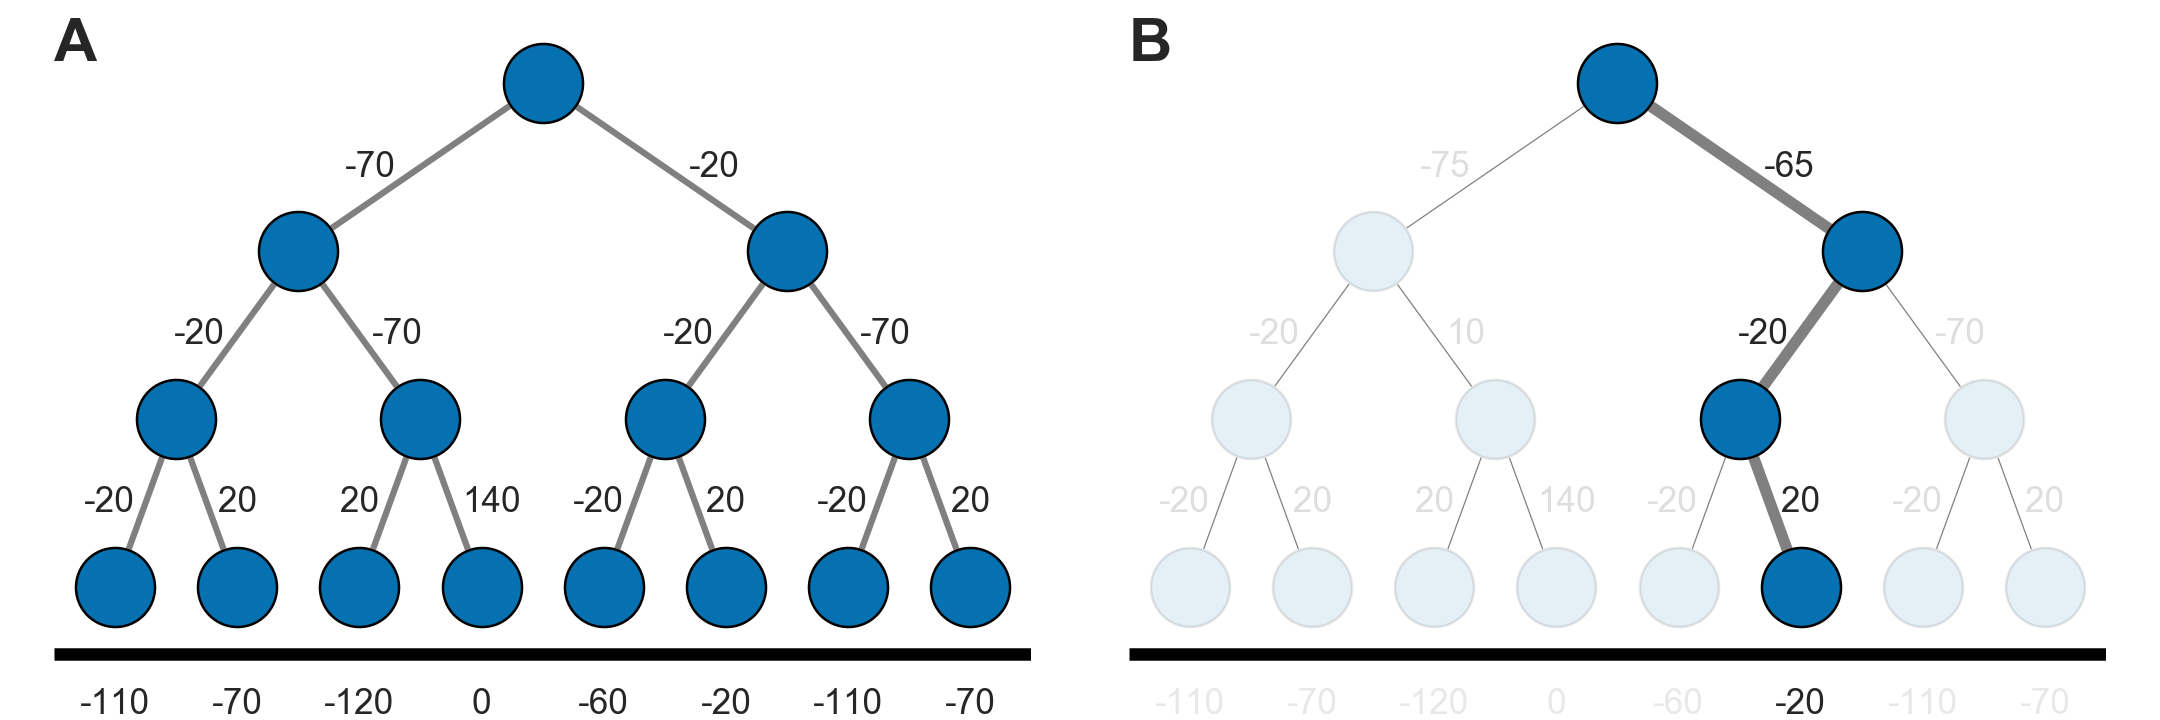
\includegraphics[trim={0 0 0 0},clip]{../../figures/04_tree_rldm.png}}%
  }
  \par \textbf{Figure 3:} (A) The decision tree environment from \cite{Huys2012} and \cite{Lally2017}. An optimistic agent ($w=1$) prefers the optimal loss-minimizing policy through the initial large loss (left branch). (B) A pessimistic agent ($w=0.5$) comes to prefer the branch without the large loss so as to avoid being unable to recoup the large initial loss. One-step rewards are presented in each state; the net value $Q$ on each path is shown numerically. (Parameters: $\gamma = 1.0$)
\end{figure}

\subsection{The anxiety-depression transition}

So far, we have considered the asymptotic preferences implied the pessimistic value function (solved for through value iteration). But we can also consider learning under this value function (e.g., by Q-learning\citep{SuttonBarto2018} or DYNA\citep{sutton1991} using the $\beta$-pessimistic return), the dynamics of which may speak to the progression of symptoms.

Of note in this respect, anxiety and depression are highly comorbid, with almost half of individuals with a lifetime depression diagnosis also diagnosed with an anxiety disorder \citep{kessler2015}. One notable proposal is that this association often arises longitudinally: in particular, that clinical anxiety precedes certain types of depression \citep{alloy1990, jacobson2014}. The idea, in brief, is that uncertainty in one's ability in the face of future threat results in anxiety and avoidance behaviors. Persistent avoidance, in turn, begets foregone reward, and ultimately to a belief that reward is unobtainable and subsequently depression. This story is borne out by simulations of learning in our model (Fig.~4) in environments like that of Fig.~1. As we observed before, the penumbra of negative value under pessimistic assumptions spreads gradually throughout the environment with the progress of learning. This in turn leads the agent to expect no reward and, echoing the anergic symptoms of depression, forego action altogether.

In addition to accounting for comorbidity of anxiety and depression, our model also hints at a reason for the longevity and recurrence of anxiety disorders even with treatment. Because pessimistic expectations allow for threat value to spread to states and actions far antecedent of the primary danger (e.g., Fig.~1d), it would accordingly also take a great many steps of iterative learning to correct all these exaggerated appraisals of threat. Frustratingly, these biased estimates of value may still remain even after a misbelief in the efficacy of future action is corrected for in a course of therapy. This may offer at least a partial answer to a classic puzzle in pathological avoidance, i.e. why it is so resistant to extinction \cite{moutoussis2018}, and to the unfortunately high rates of anxiety recurrence following treatment\citep{pittig2018}.

\begin{figure}[!b]
  \centerline{%
    \resizebox{1.0\textwidth}{!}{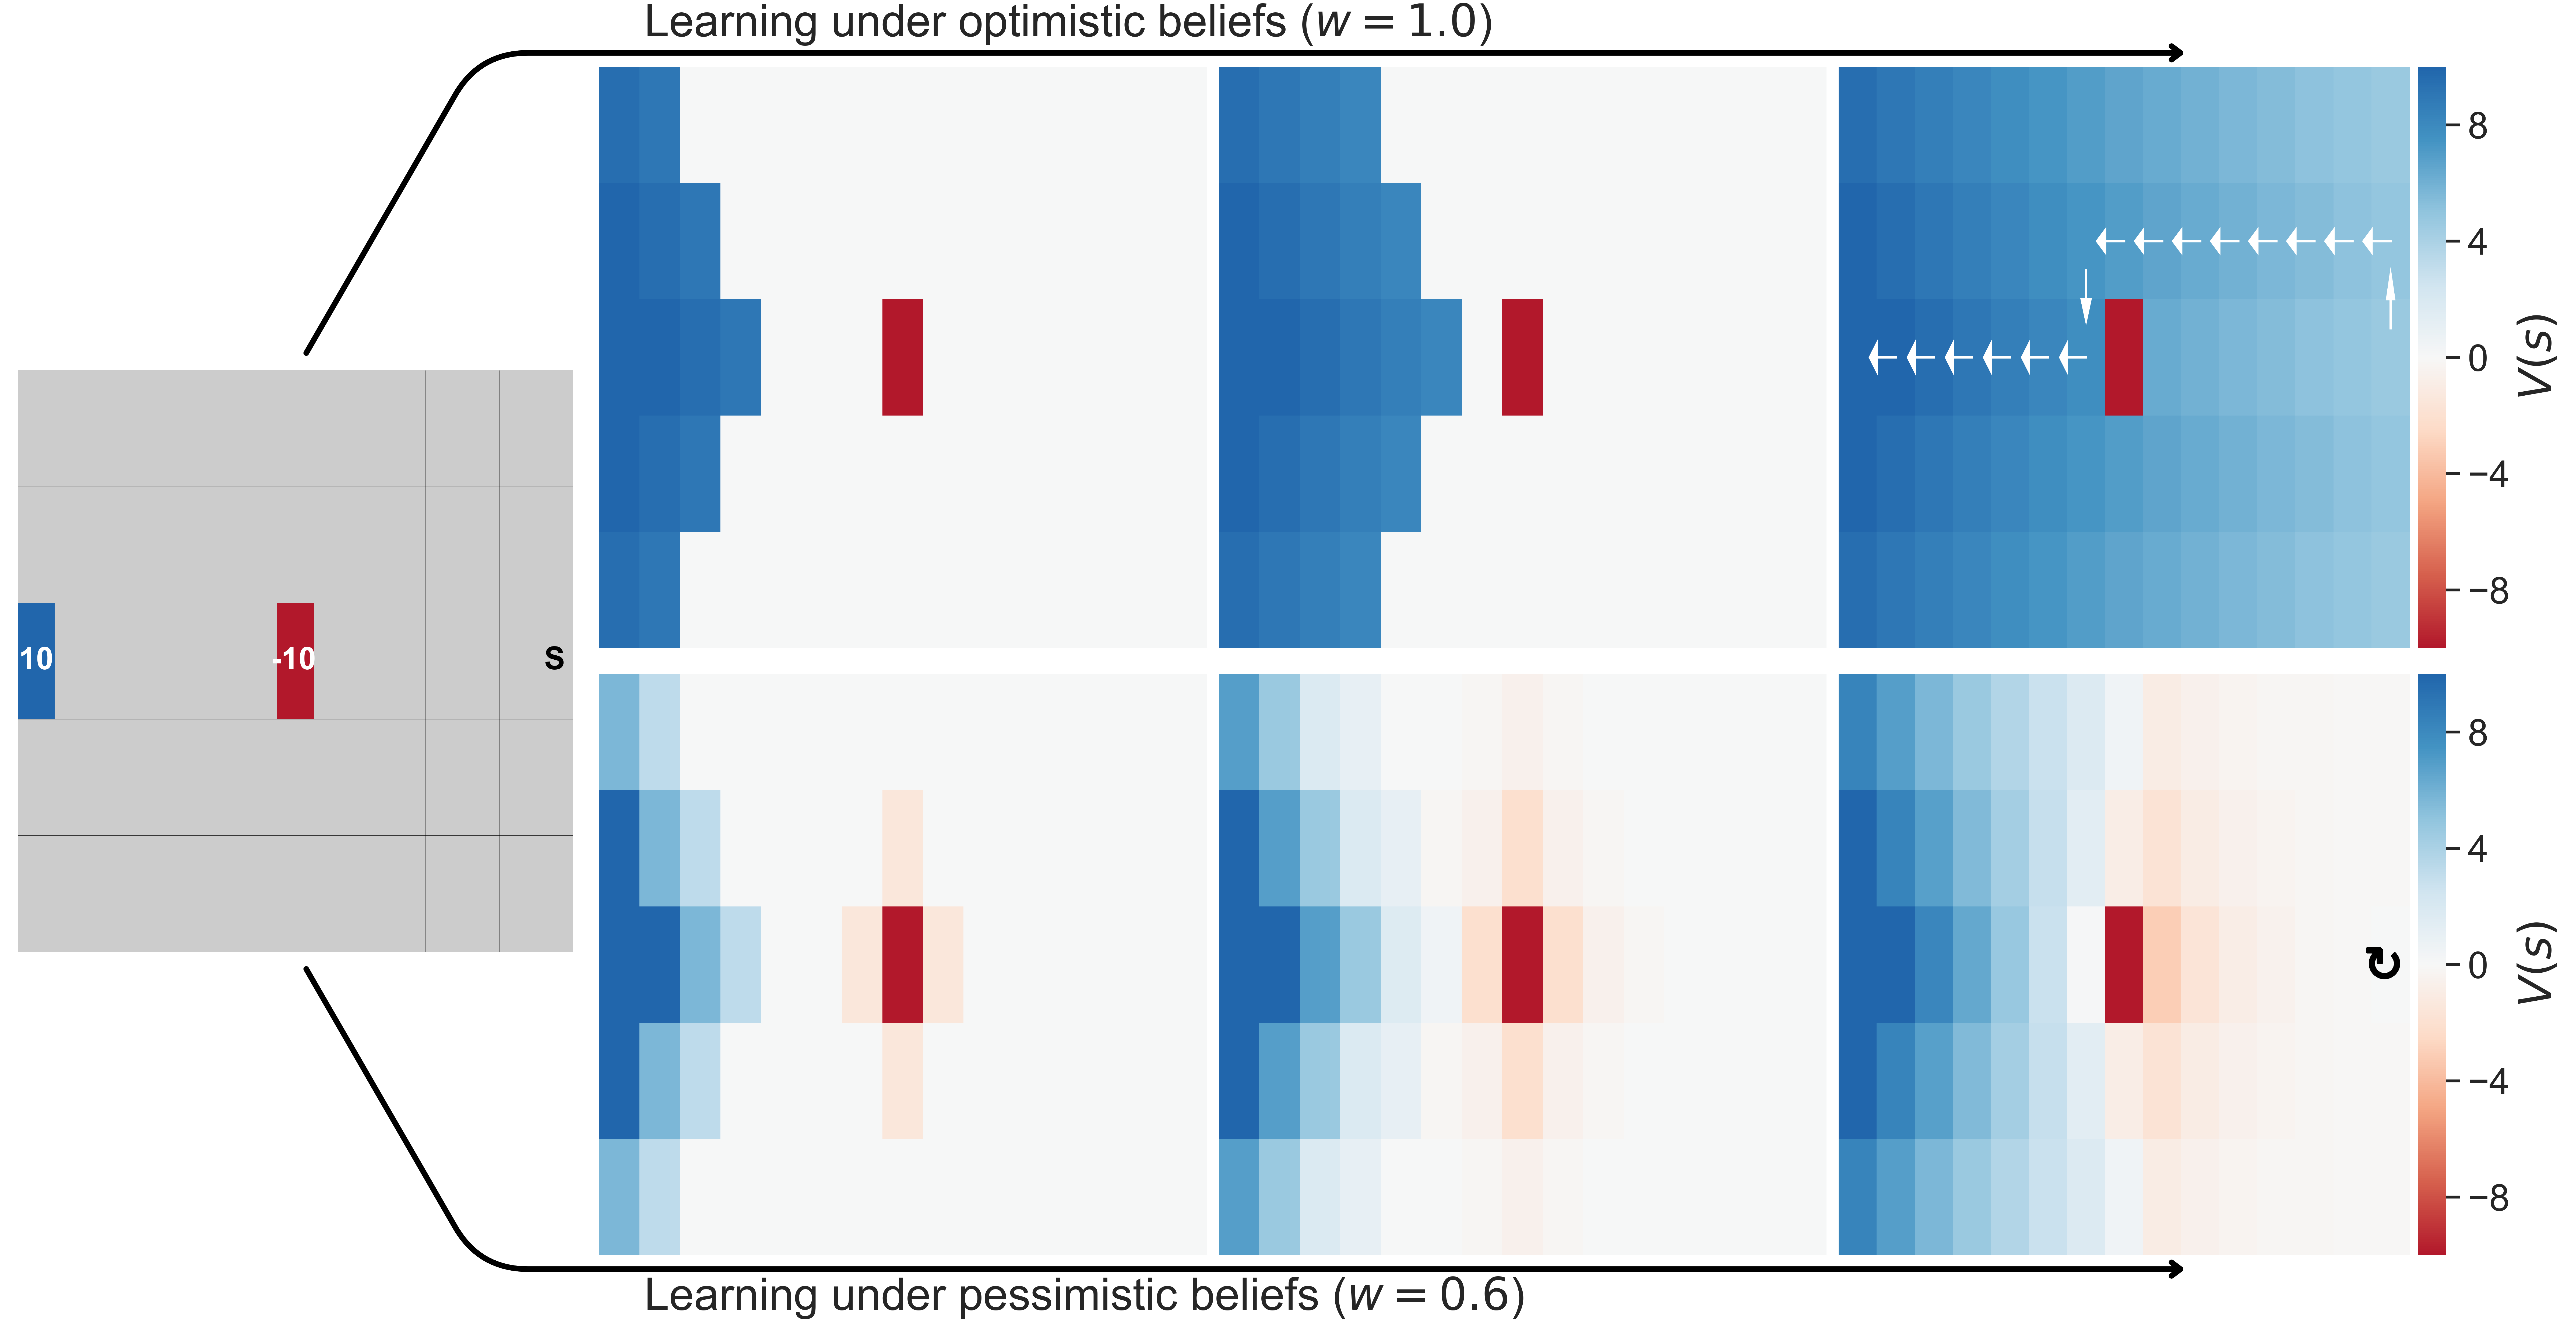
\includegraphics[trim={0 0 0 0},clip]{../../figures/03_lh.png}}%
  }
  \par \textbf{Figure 4:} A simple deterministic gridworld with two terminal states: one rewarding (blue) and one aversive (red). (B-D) States colored by their value under different levels of pessimism, with arrows showing an optimal trajectory. For an optimistic agent ($w=1$), all states (other than the harmful state) take on positive value with learning. (E-G) For a pessimistic agent ($w=0.6$), negative value spreads from the source to antecedent states. As a result of avoidance, the agent learns reward is unobtainable and develops anergic symptoms (i.e. foregoes action). (Parameters: $\gamma = 0.95$)
\end{figure}

\subsection{Free choice premium}

In this final section, we offer a novel prediction regarding the free choice premium. Simply put, the free choice premium phenomenon predicts that, all else being equal, options which lead to more choice opportunities in the future are more valuable than those that lead to fewer future choice opportunities. A free choice premium has been observed in multiple behavioral experiments \cite{Leotti2010, ly2019}. A variant of a free choice premium paradigm from \cite{Leotti2011} and \cite{Leotti2014} is presented in Fig. 5a. In the task, participants repeated choose between a free choice option, allowing for an additional future choice, and a fixed choice option; importantly, both choices lead to identical, stochastic outcomes (e.g. 50/50 chance of [1, -1]). Previous studies have found a preference for the free choice option despite it conferring no additional benefits relative to the fixed choice option. 

\begin{figure}[!b]
  \centerline{%
    \resizebox{1.0\textwidth}{!}{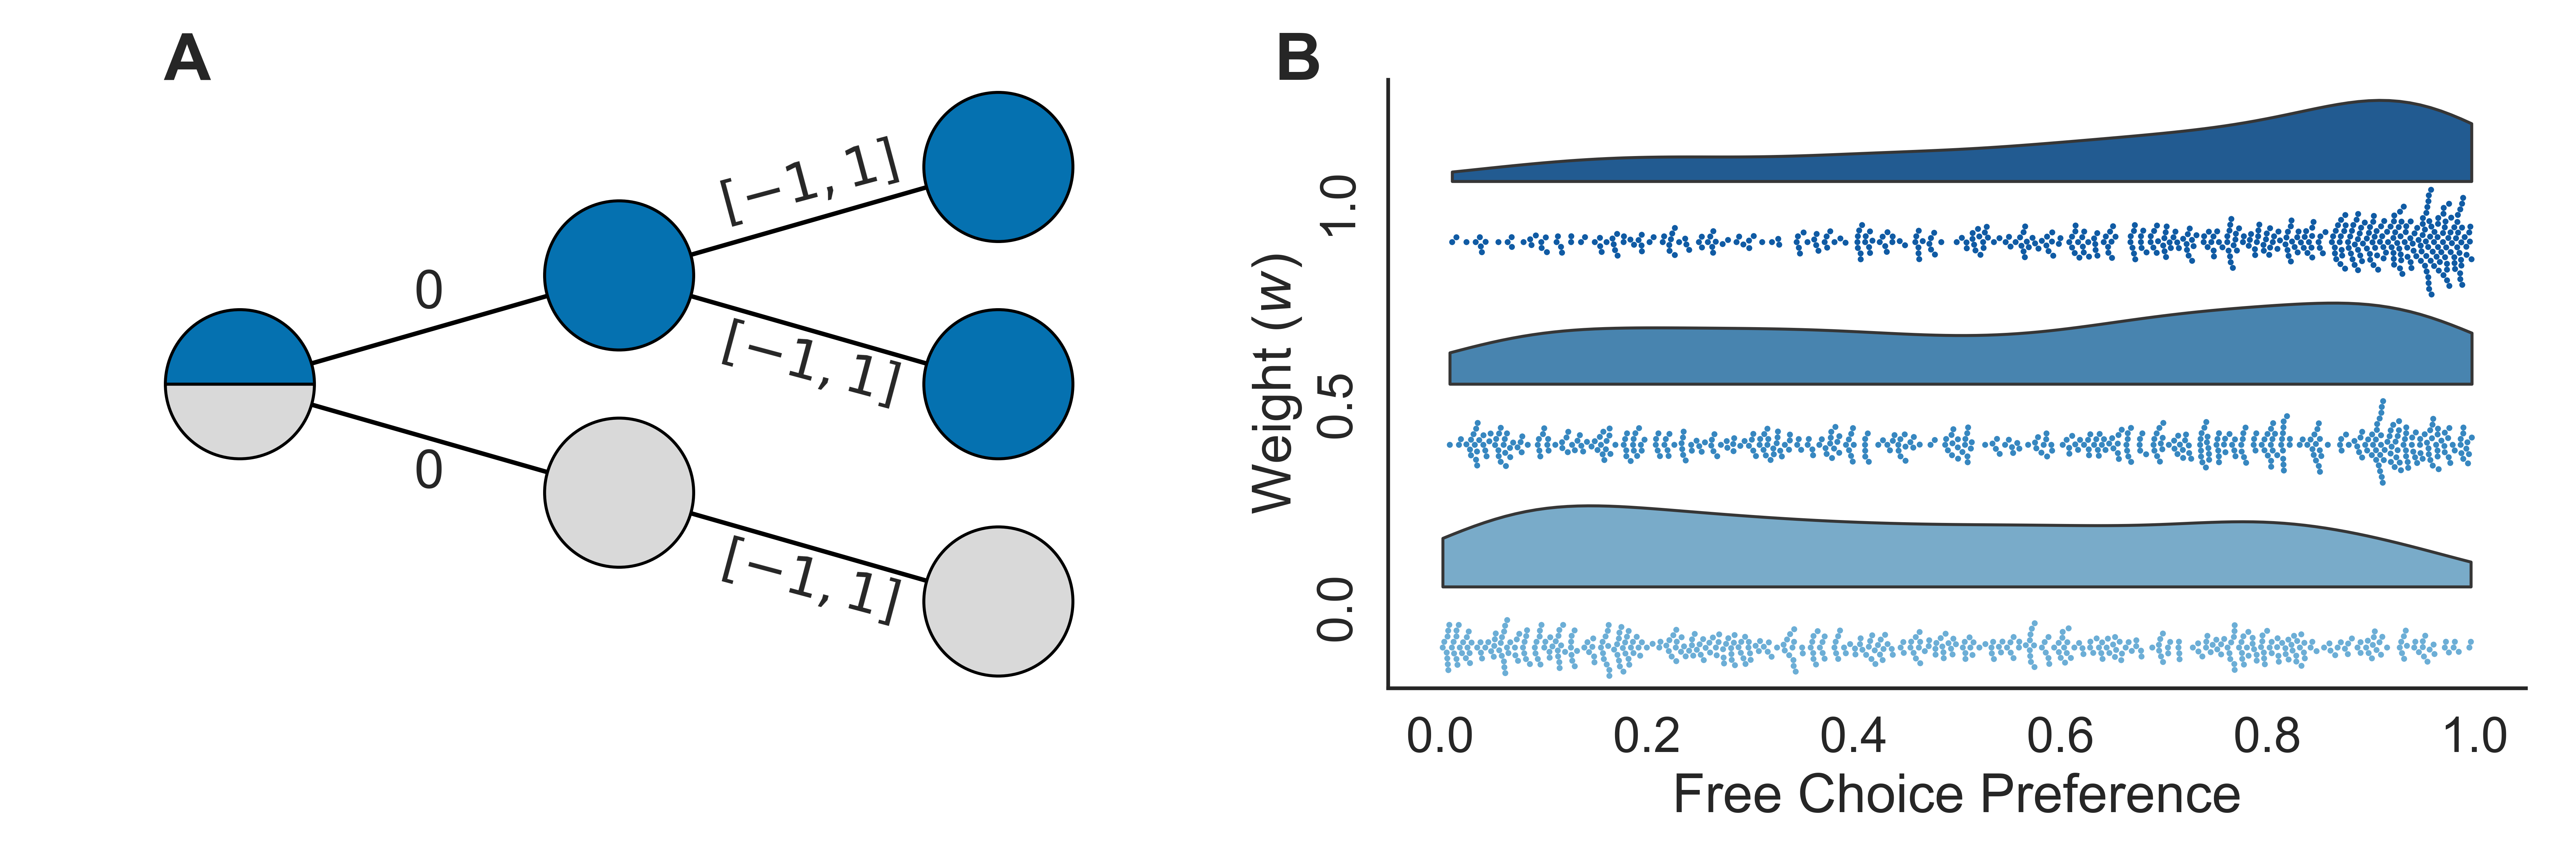
\includegraphics[trim={0 0 0 0},clip]{../../figures/05_choice.png}}%
  }
  \par \textbf{Figure 4:} (A) The free choice premium paradigm from \cite{Leotti2011} and \cite{Leotti2014} with equal chance of outcome $R \in [1, -1]$. Non-anxious participants exhibit a preference for the free choice option (blue) despite it conferring no benefit over the fixed choice option (grey). (B) Pessimistic agents show an attenuated free choice bias. (Parameters: Q-learning with $\gamma = 1.0$, and inverse temperature, $\beta$, increased from 1 to 10 over 100 episodes. Each dot represents one of 500 simulated agents.)
\end{figure}

We (and others)\citep{ly2019} suspect the free choice premium reflects the usual assumption about choice (i.e. an agent will continue to make reward-maximizing choices in the future). Under such an optimistic assumptions, additional options are valuable insofar that they allow for additional future reward opportunities (or, at the worst, pose no possible harm). On the contrary, if anxiety reflects a violation of this typical assumption, then we should suspect anxious individuals will exhibit a diminished free choice bias. Indeed, the model makes this prediction (Fig. ~5b). We plan on explicitly testing this hypothesis in subclinical and clinical anxiety in the near future.

\section{Discussion}

Central to anxiety disorders are symptoms including exaggerated threat appraisal, threat generalization, and excessive avoidance. We have presented a simple computational account suggesting how a single underlying misbelief can give rise to these aberrations in learning and choice. Specifically, we showed how a failure to believe in the reliability of future self-action can effectively backpropagate negative value across states of the environment. This process results in a range of inferences and behaviors resembling those observed in clinical anxiety. Though this is by no means a complete account of anxiety, it ties together a surprisingly wide range of its symptoms.

One important ambiguity is that we have formalized pessimistic assumptions in terms of beliefs about the agent's own future actions: expecting failure in handling or avoiding future threat. Since Eq.~1 is also computed in expectation over the anticipated future environmental dynamics $p(s' \mid s,a)$, pessimism can alternatively be encoded in this distribution (e.g., a belief that the world's response to one's choices is unpredictable or adversarial). Because the Bellman equation averages out both distributions, and because an unpredictable environment also reduces the efficacy of avoidance, either formulation can produce ultimately similar results. However from the perspective of cognitive theories of anxiety, these represent quite different maladaptive beliefs, which may be relevant, for instance, in guiding treatment.

Indeed, our account formalizes a longstanding strand of theory on the role of control in anxiety. Central to many prominent cognitive theories of anxiety in the psychiatric literature is a perceived lack of control. For example, self-efficacy theory\citep{bandura1977} and the triple vulnerabilities model\citep{barlow2002} both posit that a reduced belief in the ability to effectively respond to future threat is involved in the genesis and maintenance of clinical anxiety. Similarly, the learned helplessness theories of anxiety\cite{alloy1990} claims clinical anxiety results from an uncertain belief in the controllability of the environment, such that future threat cannot be effectively mitigated or avoided. As we note above, the present model (though stated here in terms of self-efficacy) can accommodate either variant, and they are by no means mutually exclusive.

Distortions in beliefs about future action or transition probabilities are in no way the only means through which anxious behaviors may arise in a decision theoretic account. Traditionally, the goal of reinforcement learning algorithms is to a find reward-maximizing policy with respect to the expectation (average) of returns. However, in environments where the distribution of returns has high variance, such that there is potential for catastrophic loss, it may be instead preferable to learn a policy with respect to an alternative value function. The same is true when there is uncertainty in the transition probabilities, such that an agent may inadvertently step towards undesirable and/or dangerous segments of the environment. How to learn risk-sensitive and robust policies is the focus of much recent research \cite{morimura2012, chow2015, bellemare2017}; interestingly, these studies have reported agent behaviors not unlike those presented here. It is important to note that anxiety is correlated with disproportionate worry about low chance but high cost events\cite{Miceli2005}. One speculative hypothesis is that anxious individuals learn and evaluate action with respect  to a more pessimistic point in the distribution of expected returns.

A separate possibility concerns the notion of state. In the present work, we considered only environments with fully observable states; in other words, there was no uncertainty regard the state an agent was currently occupying. In the real-world, however, the state must be inferred from external and internal observations. One possibility is that anxiety is a function of biases in state inference\cite{Paulus2012}. For example, if an agent erroneously comes to the conclusion that she is more proximal to threat than is actually the case, then symptoms like exaggerated threat appraisal and avoidance should arise. Indeed, a bias in value functions could result in the diffuse spread of threat across objects\citep{norbury2018} and location\citep{schulz2018}, thereby causing otherwise benign states to be perceived as threatening. 

% not sure if this paragraph is good

None of the previous discussion constitutes a claim about the algorithmic and neural bases of pessimistic sequential evaluation. One possibility is that these symptoms reflect aberrations in model-based planning. Model-based planning refers to the process of sequentially evaluation of trajectories of action, which may go awry in anxiety if successful avoidance actions are discounted or otherwise downweighted. Chronic worry is a symptom frequently observed in clinical anxiety, and bears resemblance to aberrant model-based planning wherein the trajectories are biased towards bad- or worst-case contingencies. In line with the present results, chronic worry is associated with reduced perceived control, diminished belief in self-efficacy in response to threat, and exaggerated threat appraisal\cite{Berenbaum2010}. This suggests that clinical anxiety may in part result from planning processes gone awry. 

A second possibility is that pessimistic evaluation may arise as a result of biased offline replay of events. During periods of rest and sleep, the hippocampus replays recent experiences\citep{whats a good ref?}. A recent theoretical model of replay suggests that these replay events are able to iteratively backpropagate value from a focal point to antecedent states, and that episodes are prioritized for replay according to their likelihood in changing behavior. Biases in replay behavior, or in the mechanisms initiate replay, might result in repeated offline reinforcement of negative episodes thereby exaggerating the value of threat and diffusing its influence across an agent's internal cognitive map. Few studies have investigated replay behavior in aversive environments (e.g. \citep{wu2017}), so this hypothesis remains speculative at this point in time.   

%% Want to add anything about transition probability bias?

It is important to note that the present model may not describe all anxiety disorders with equal accuracy. Indeed, our model of pessimistic sequential evaluation is, by definition, a model of prospective cognition. As such, the present results are more likely to accurately describe the anxiety disorders which primarily involve aberrations in future-oriented cognitive processes, such as generalized and social anxiety disorders. Naturally, the present model can neither account for the compulsive behaviors of obsessive-compulsive disorder nor the memory disturbances of post-traumatic stress disorder (though recent clinical studies suggest that diminished perceived control is a vulnerability factor common to all anxiety disorders, including OCD and PTSD)\citep{gallagher2014a, gallagher2014b}. Importantly, other psychiatric disorders that involve future-oriented misbeliefs, worry, and avoidance behaviors (e.g. eating disorders\citep{konstantellou2011}) may similarly be well-described by the current account. As such, the present results are transdiagnostic and not limited to one particular diagnosis. 

Finally, we are not the first to propose a formal theory of control in psychiatry using MDPs. Huys \& Dayan \cite{HuysDayan2009} also provided a computational account of learned helplessness through simple models of one-step action-outcome contingencies. Our accounts differ particularly in our exclusive focus on control in the sequential setting, which Huys \& Dayan did not address. Indeed, we propose that ultimately key to anxiety is precisely the way in which evaluation in sequential tasks is necessarily reliant on expectations about future choice and events.

\bibliographystyle{naturemag}
\small{\bibliography{manuscript}}

\end{document}
